\documentclass{beamer}
\usetheme{Singapore}
\usepackage[utf8]{inputenc}
\usecolortheme{crane}
\usepackage{graphicx}
\usepackage{iwona}
\usepackage{standalone}
\usepackage{tikz}
\usetikzlibrary{arrows}
\usetikzlibrary{decorations.markings}
\usetikzlibrary{calc}
\usetikzlibrary{shapes,snakes}
\usepackage{amsmath}
\usepackage{amsfonts}
\usepackage{amsthm}
\usepackage{mathtools}
\usepackage{tcolorbox}
\usepackage{listings}
\usepackage{float}
\usepackage{bm}

\definecolor{lightblue}{RGB}{124,190,255}
\definecolor{darkgreen}{RGB}{24,145,0}
\definecolor{darkorange}{RGB}{220,110,0}
\definecolor{codegreen}{RGB}{0,120,0}

\lstset{language=Python,
basicstyle=\scriptsize\ttfamily\bfseries,
commentstyle=\color{red}\itshape,
stringstyle=\color{darkorange},
showstringspaces=false,
keywordstyle=\color{codegreen}\bfseries}



\beamertemplatenavigationsymbolsempty
\setbeamerfont{caption}{size=\tiny}


\title
{ASQ Simulates Queues}
\author{Geraint Palmer}
\date{PyCon Namibia 2016}
\titlegraphic{
\includegraphics[width=2.5cm]{cflogo} $\quad$ 
\includegraphics[width=2.5cm]{asq_logo} $\quad$ 
\includegraphics[width=2.5cm]{napycon_logo}}



\begin{document}

\frame{\titlepage}

\begin{frame}
\frametitle{What is a Queue?}
\begin{figure}
  \includestandalone[width=0.8\textwidth]{1nodeexample}
\end{figure}
\end{frame}

\begin{frame}
\frametitle{What is a Queue?}
\begin{figure}
  \includestandalone[width=0.8\textwidth]{2nodefeedbackexample}
\end{figure}
\end{frame}

\begin{frame}
\begin{figure}
    \includestandalone[width=0.35\textwidth]{repostructure_scripts}
\end{figure}
\end{frame}

\begin{frame}
\frametitle{Demo}
\begin{figure}
    
\includegraphics[width=0.7\textwidth]{asq_logo}
\end{figure}
\end{frame}

\begin{frame}
\begin{figure}
    \includestandalone[width=0.35\textwidth]{repostructure_code}
\end{figure}
\end{frame}

\begin{frame}
\frametitle{Three-Phase Simulation Approach}
\begin{figure}
    \includestandalone[width=\textwidth]{3phaseapprach}
\end{figure}
\end{frame}

\begin{frame}
\frametitle{Event Types}
\begin{figure}
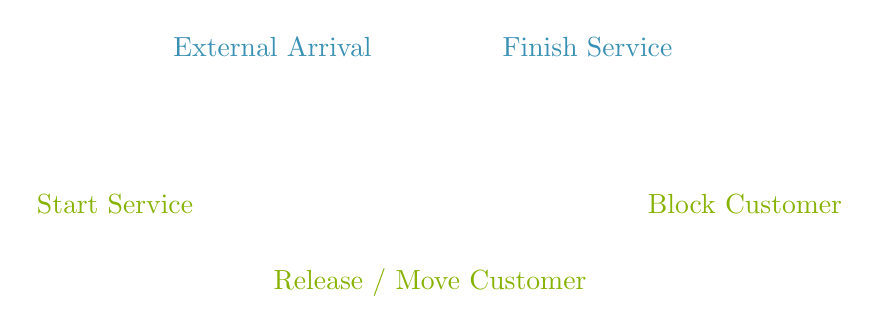
\begin{tikzpicture}
\node[text=cyan!70!black] at (0, 0) {External Arrival};
\node[text=cyan!70!black] at (4, 0) {Finish Service};
\node[text=lime!70!black] at (-2, -2) {Start Service};
\node[text=lime!70!black] at (2, -3) {Release / Move Customer};
\node[text=lime!70!black] at (6, -2) {Block Customer};
\end{tikzpicture}
\end{figure}
\end{frame}

\begin{frame}
\frametitle{Code Structure}
\begin{figure}
    \includestandalone[width=\textwidth]{codestructure}
\end{figure}
\end{frame}

\begin{frame}
\frametitle{Pair Programing / Collaborative Work}
\end{frame}

\begin{frame}
\frametitle{Git \& GitHub}
\end{frame}

\begin{frame}
\frametitle{GitHub Issues}
\begin{figure}
    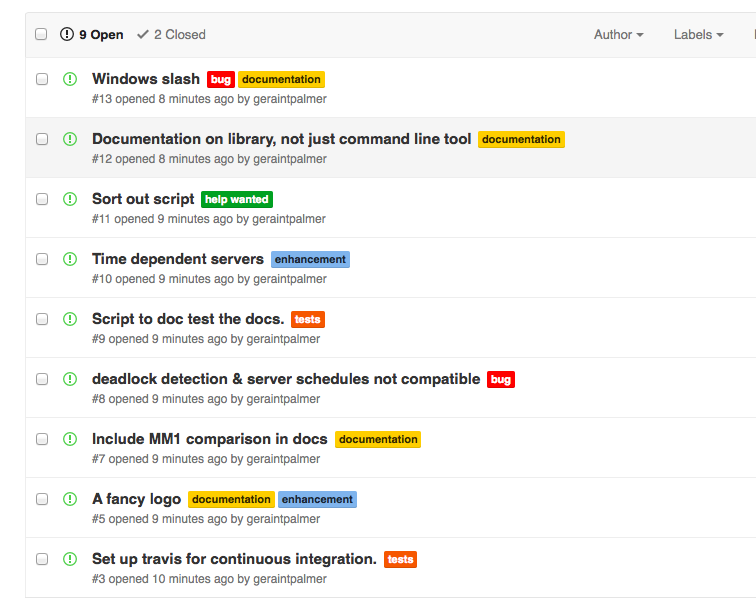
\includegraphics[width=0.8\textwidth]{githubissues}
\end{figure}
\end{frame}

\begin{frame}
\begin{figure}
    \includestandalone[width=0.35\textwidth]{repostructure_tests}
\end{figure}
\end{frame}

\begin{frame}
\frametitle{Doctests}
\resizebox{\textwidth}{!}{%
\lstinputlisting[language=Python]{doctests.py}%
}
\end{frame}

\begin{frame}
\frametitle{Unittests}
\resizebox{\textwidth}{!}{%
\lstinputlisting[language=Python]{unittests.py}%
}
\end{frame}

\begin{frame}
\frametitle{Travis}
\end{frame}

\begin{frame}
\begin{figure}
    \includestandalone[width=0.35\textwidth]{repostructure_packaging}
\end{figure}
\end{frame}

\begin{frame}
\frametitle{Packaging}
\end{frame}

\begin{frame}
\begin{figure}
    \includestandalone[width=0.35\textwidth]{repostructure_docs}
\end{figure}
\end{frame}

\begin{frame}
\frametitle{Documentation}
\end{frame}


\begin{frame}
\frametitle{Academic Uses}
\vfill
\begin{block}{Theoretical Work}
Investigating deadlock in queueing networks.\\
(Geraint Palmer, Prof. Paul Harper, Dr. Vincent Knight)
\end{block}
\vfill
\begin{block}{Practical Work}
Modelling an ophthalmology clinic to strategise scheduling.\\
(Lieke H\"{o}lscher, Dr. Jennifer Morgan)
\end{block}
\vfill
\end{frame}


\begin{frame}
\frametitle{Investigating Deadlock}
\begin{figure}
    \includestandalone[width=\textwidth]{deadlock_digraph}
\end{figure}
\end{frame}

\begin{frame}
\begin{figure}
    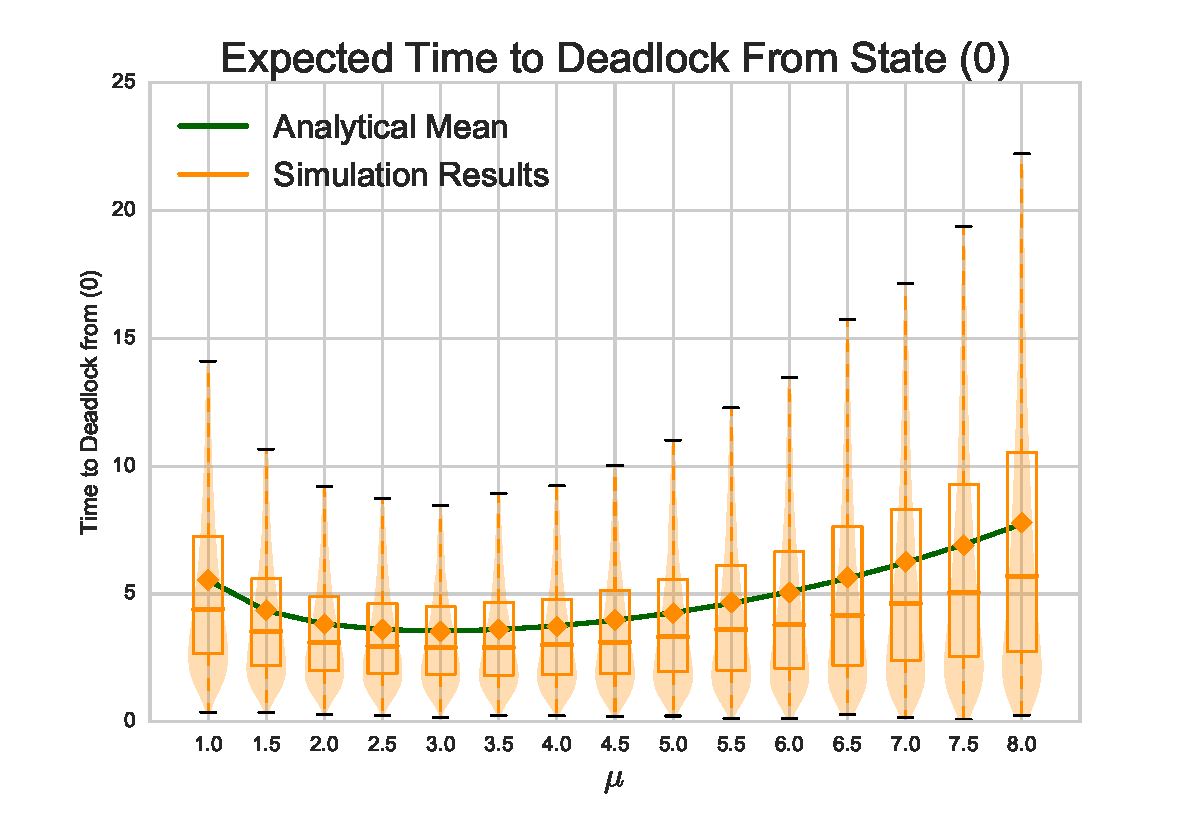
\includegraphics[width=\textwidth]{varymu_1Nms}
\end{figure}
\end{frame}

\begin{frame}
\frametitle{Modelling Ophthalmology Clinic}
\begin{figure}
    \includestandalone[width=0.9\textwidth]{ophthalmology}
\end{figure}
\end{frame}

\end{document}
